\subsection{Describing non-discoverable hardware: Device Tree}

\begin{frame}{Describing non-discoverable hardware}
  \begin{columns}
    \column{0.3\textwidth}
    \begin{enumerate}
    \item<1> Directly in the {\bf OS/bootloader code}
    \item<2> Using {\bf ACPI} tables
    \item<3> Using a {\bf Device Tree}
    \end{enumerate}
    \column{0.7\textwidth}
    \only<1> {
      \begin{itemize}
      \item Using compiled data structures, typically in C
      \item How it was done on most embedded platforms in Linux, U-Boot.
      \item Considered not maintainable/sustainable on ARM32, which
        motivated the move to another solution.
      \end{itemize}
    }
    \only<2> {
      \begin{itemize}
      \item On {\em x86} systems, but also on a subset of ARM64 platforms
      \item Tables provided by the firmware
      \end{itemize}
    }
    \only<3> {
      \begin{itemize}
      \item Originates from {\bf OpenFirmware}, defined by Sun, used on
        SPARC and PowerPC
        \begin{itemize}
        \item That's why many Linux/U-Boot functions related to DT have
          a \code{of_} prefix
        \end{itemize}
      \item Now used by most embedded-oriented CPU architectures that run
        Linux: ARC, ARM64, RISC-V, ARM32, PowerPC, Xtensa, MIPS, etc.
      \item Writing/tweaking a DT is necessary when porting Linux to a
        new board, or when connecting additional peripherals
      \end{itemize}
    }
  \end{columns}
\end{frame}

\begin{frame}{Device Tree: from source to blob}
  \begin{columns}
    \column{0.7\textwidth}
    \begin{itemize}
    \item A tree data structure describing the hardware is written by a
      developer in a {\bf Device Tree Source} file, \code{.dts}
    \item Processed by the {\bf Device Tree Compiler}, \code{dtc}
    \item Produces a more efficient representation: {\bf Device Tree
        Blob}, \code{.dtb}
    \item Additional C preprocessor pass
    \item \code{.dtb} $\rightarrow$ accurately describes the hardware platform in an {\bf OS-agnostic} way.
    \item \code{.dtb} $\approx$ few dozens of kilobytes
    \item DTB also called {\bf FDT}, {\em Flattened Device Tree}, once
      loaded into memory.
      \begin{itemize}
      \item \code{fdt} command in U-Boot
      \item \code{fdt_} APIs
      \end{itemize}
    \end{itemize}
    \column{0.3\textwidth}
    \includegraphics[height=0.7\textheight]{slides/linux-kernel-access-hw-dt/dts-to-dtb.pdf}
  \end{columns}
\end{frame}

\begin{frame}[fragile]{dtc example}
  \footnotesize
  \begin{columns}[t]
    \column{0.5\textwidth}
    \begin{block}{}
\begin{verbatim}
$ cat foo.dts
/dts-v1/;

/ {
        welcome = <0xBADCAFE>;
        bootlin {
                webinar = "great";
                demo = <1>, <2>, <3>;
        };
};
\end{verbatim}
    \end{block}
    \pause
    \begin{block}{}
\begin{verbatim}
$ dtc -I dts -O dtb -o foo.dtb foo.dts
$ ls -l foo.dt*
-rw-r--r-- 1 thomas thomas 169 ... foo.dtb
-rw-r--r-- 1 thomas thomas 102 ... foo.dts
\end{verbatim}
    \end{block}
    \pause
    \column{0.5\textwidth}
    \begin{block}{}
\begin{verbatim}
$ dtc -I dtb -O dts foo.dtb
/dts-v1/;

/ {
        welcome = <0xbadcafe>;

        bootlin {
                webinar = "great";
                demo = <0x01 0x02 0x03>;
        };
};
\end{verbatim}
    \end{block}
  \end{columns}
\end{frame}

\begin{frame}{Device Tree: using the blob}
  \begin{columns}
    \column{0.6\textwidth}
    \begin{itemize}
    \item Can be {\bf linked directly} inside a bootloader binary
      \begin{itemize}
      \item For example: U-Boot, Barebox
      \end{itemize}
    \item Can be {\bf passed} to the operating system by the bootloader
      \begin{itemize}
      \item Most common mechanism for the Linux kernel
      \item U-Boot: \code{boot[z,i,m] <kernel-addr> - <dtb-addr>}
      \item The bootloader can adjust the DTB before passing it to the
        kernel
      \end{itemize}
    \item The DTB parsing can be done using \code{libfdt}, or ad-hoc
      code
    \end{itemize}
    \column{0.4\textwidth}
    \includegraphics[height=0.8\textheight]{slides/linux-kernel-access-hw-dt/ram.pdf}
  \end{columns}
\end{frame}

\begin{frame}{Where are Device Tree Sources located?}
  \begin{itemize}
  \item Even though they are OS-agnostic, {\bf no central and
      OS-neutral} place to host Device Tree sources and share them
    between projects
    \begin{itemize}
    \item Often discussed, never done
    \end{itemize}
  \item In practice, the Linux kernel sources can be considered as the
    {\bf canonical location} for Device Tree Source files
    \begin{itemize}
    \item \code{arch/<ARCH>/boot/dts/<vendor>/}
    \item \code{arch/arm/boot/dts} (on ARM 32 architecture before Linux 6.5)
    \item $\approx$ 4500 Device Tree Source files (\code{.dts} and
          \code{.dtsi}) in Linux as of 6.0.
    \end{itemize}
  \item Duplicated/synced in various projects
    \begin{itemize}
    \item U-Boot, Barebox, TF-A
    \end{itemize}
  \end{itemize}
\end{frame}

\begin{frame}{Device Tree base syntax}
  \begin{columns}
    \column{0.5\textwidth}
    \begin{itemize}
    \item Tree of {\bf nodes}
    \item Nodes with {\bf properties}
    \item Node $\approx$ a device or IP block
    \item Properties $\approx$ device characteristics
    \item Notion of {\bf cells} in property values
    \item Notion of {\bf phandle} to point to other nodes
    \item \code{dtc} only does syntax checking, no semantic validation
    \end{itemize}
    \column{0.5\textwidth}
    \begin{center}
      \includegraphics[height=0.6\textheight]{slides/linux-kernel-access-hw-dt/dt-basic-syntax.pdf}
    \end{center}
  \end{columns}
\end{frame}

\begin{frame}[fragile]{DT overall structure: simplified example}
  \begin{columns}
    \column{0.6\textwidth}
    \begin{onlyenv}<1>
      \begin{block}{}
\begin{minted}[fontsize=\tiny]{perl}
/ {
  #address-cells = <1>;
  #size-cells = <1>;
  model = "STMicroelectronics STM32MP157C-DK2 Discovery Board";
  compatible = "st,stm32mp157c-dk2", "st,stm32mp157";

  cpus { ... };
  memory@0 { ... };
  chosen { ... };
  intc: interrupt-controller@a0021000 { ... };
  soc {
    i2c1: i2c@40012000 { ... };
    ethernet0: ethernet@5800a000 { ... };
  };
};
\end{minted}
      \end{block}
    \end{onlyenv}
    \begin{onlyenv}<2>
      \begin{block}{}
\begin{minted}[fontsize=\tiny]{perl}
/ {
  cpus {
    #address-cells = <1>;
    #size-cells = <0>;
    cpu0: cpu@0 {
      compatible = "arm,cortex-a7";
      clock-frequency = <650000000>;
      device_type = "cpu";
      reg = <0>;
    };

    cpu1: cpu@1 {
      compatible = "arm,cortex-a7";
      clock-frequency = <650000000>;
      device_type = "cpu";
      reg = <1>;
    };
  };

  memory@0 { ... };
  chosen { ... };
  intc: interrupt-controller@a0021000 { ... };
  soc {
    i2c1: i2c@40012000 { ... };
    ethernet0: ethernet@5800a000 { ... };
  };
};
\end{minted}
      \end{block}
    \end{onlyenv}
    \begin{onlyenv}<3>
      \begin{block}{}
\begin{minted}[fontsize=\tiny]{perl}
/ {
  cpus { ... };
  memory@0 {
    device_type = "memory";
    reg = <0x0 0x20000000>;
  };

  chosen {
    bootargs = "";
    stdout-path = "serial0:115200n8";
  };
  intc: interrupt-controller@a0021000 { ... };
  soc {
    i2c1: i2c@40012000 { ... };
    ethernet0: ethernet@5800a000 { ... };
  };
};
\end{minted}
      \end{block}
    \end{onlyenv}
    \begin{onlyenv}<4>
      \begin{block}{}
\begin{minted}[fontsize=\tiny]{perl}
/ {
  cpus { ... };
  memory@0 { ... };
  chosen { ... };

  intc: interrupt-controller@a0021000 {
    compatible = "arm,cortex-a7-gic";
    #interrupt-cells = <3>;
    interrupt-controller;
    reg = <0xa0021000 0x1000>,
          <0xa0022000 0x2000>;
  };

  soc {
    compatible = "simple-bus";
    #address-cells = <1>;
    #size-cells = <1>;
    interrupt-parent = <&intc>;

    i2c1: i2c@40012000 { ... };
    ethernet0: ethernet@5800a000 { ... };
  };
};
\end{minted}
      \end{block}
    \end{onlyenv}
    \begin{onlyenv}<5>
      \begin{block}{}
\begin{minted}[fontsize=\tiny]{perl}
/ {
  cpus { ... };
  memory@0 { ... };
  chosen { ... };
  intc: interrupt-controller@a0021000 { ... };
  soc {
    i2c1: i2c@40012000 {
      compatible = "st,stm32mp15-i2c";
      reg = <0x40012000 0x400>;
      interrupts = <GIC_SPI 31 IRQ_TYPE_LEVEL_HIGH>,
                   <GIC_SPI 32 IRQ_TYPE_LEVEL_HIGH>;
      #address-cells = <1>;
      #size-cells = <0>;
      status = "okay";

      cs42l51: cs42l51@4a {
        compatible = "cirrus,cs42l51";
        reg = <0x4a>;
        reset-gpios = <&gpiog 9 GPIO_ACTIVE_LOW>;
        status = "okay";
      };
    };
    ethernet0: ethernet@5800a000 { ... };
  };
};
\end{minted}
      \end{block}
    \end{onlyenv}
    \begin{onlyenv}<6>
      \begin{block}{}
\begin{minted}[fontsize=\tiny]{perl}
/ {
  cpus { ... };
  memory@0 { ... };
  chosen { ... };
  intc: interrupt-controller@a0021000 { ... };
  soc {
    compatible = "simple-bus";
    ...
    interrupt-parent = <&intc>;
    i2c1: i2c@40012000 { ... };

    ethernet0: ethernet@5800a000 {
      compatible = "st,stm32mp1-dwmac", "snps,dwmac-4.20a";
      reg = <0x5800a000 0x2000>;
      interrupts-extended = <&intc GIC_SPI 61 IRQ_TYPE_LEVEL_HIGH>;
      status = "okay";

      mdio0 {
        #address-cells = <1>;
        #size-cells = <0>;
        compatible = "snps,dwmac-mdio";
        phy0: ethernet-phy@0 {
          reg = <0>;
        };
      };
    };
  };
};
\end{minted}
      \end{block}
    \end{onlyenv}
    \column{0.4\textwidth}
    \includegraphics[width=\textwidth]{slides/linux-kernel-access-hw-dt/simple-hardware.pdf}
  \end{columns}
\end{frame}

\begin{frame}[fragile]{Device Tree inheritance}
  \begin{itemize}
  \item Device Tree files are not monolithic, they can be split in
    several files, including each other.
  \item \code{.dtsi} files are included files, while \code{.dts} files
    are {\em final} Device Trees
    \begin{itemize}
    \item Only \code{.dts} files are accepted as input to \code{dtc}
    \end{itemize}
  \item Typically, \code{.dtsi} will contain
    \begin{itemize}
    \item definitions of SoC-level information
    \item definitions common to several boards
    \end{itemize}
  \item The \code{.dts} file contains the board-level information
  \item The inclusion works by {\bf overlaying} the tree of the
    including file over the tree of the included file,
    according to the order of the \code{#include} directives.
  \item Allows an including file to {\bf override} values specified by
    an included file
  \item Uses the C pre-processor \code{#include} directive
  \end{itemize}
\end{frame}

\begin{frame}{Device Tree inheritance example}
  \begin{center}
    \includegraphics[width=\textwidth]{slides/linux-kernel-access-hw-dt/dt-inheritance.pdf}
  \end{center}
\end{frame}

\begin{frame}[fragile]{Inheritance and labels}

  \begin{columns}[t]
    \column{0.5\textwidth}
    Doing:
    \begin{block}{soc.dtsi}
      {\tiny
\begin{minted}{perl}
/ {
  soc {
    usart1: serial@5c000000 {
      compatible = "st,stm32h7-uart";
      reg = <0x5c000000 0x400>;
      status = "disabled";
    };
  };
};
\end{minted}
      }
    \end{block}

    \begin{block}{board.dts}
      {\tiny
\begin{minted}{perl}
#include "soc.dtsi"

/ {
  soc {
    serial@5c000000 {
      status = "okay";
    };
  };
};
\end{minted}
      }
    \end{block}

    \column{0.5\textwidth}
    \begin{onlyenv}<2>
    Is exactly equivalent to:

    \begin{block}{soc.dtsi}
      {\tiny
\begin{minted}{perl}
/ {
  soc {
    usart1: serial@5c000000 {
      compatible = "st,stm32h7-uart";
      reg = <0x5c000000 0x400>;
      status = "disabled";
    };
  };
};
\end{minted}
      }
    \end{block}

    \begin{block}{board.dts}
      {\tiny
\begin{minted}{perl}
#include "soc.dtsi"

&usart1 {
  status = "okay";
};
\end{minted}
        }
      \end{block}

      $\rightarrow$ this solution is now often preferred
      \end{onlyenv}
  \end{columns}

\end{frame}

\begin{frame}{DT inheritance in STM32MP1 support}
  \begin{center}
    \includegraphics[height=0.8\textheight]{slides/linux-kernel-access-hw-dt/dt-inheritance-stm32.pdf}
  \end{center}
\end{frame}

\begin{frame}{Device Tree design principles}
  \begin{itemize}
  \item {\bf Describe hardware} (how the hardware is), not
    configuration (how I choose to use the hardware)
  \item {\bf OS-agnostic}
    \begin{itemize}
    \item For a given piece of HW, Device Tree should be the same for
      U-Boot, FreeBSD or Linux
    \item There should be no need to change the Device Tree when updating the OS
    \end{itemize}
  \item Describe {\bf integration of hardware components}, not the internals
    of hardware components
    \begin{itemize}
    \item The details of how a specific device/IP block is working is
      handled by code in device drivers
    \item The Device Tree describes how the device/IP block is
      connected/integrated with the rest of the system: IRQ lines, DMA
      channels, clocks, reset lines, etc.
    \end{itemize}
  \item Like all beautiful design principles, these principles are
    sometimes violated.
  \end{itemize}
\end{frame}

\begin{frame}{Device Tree specifications}
  \begin{columns}
    \column{0.7\textwidth}
    \begin{itemize}
    \item How to write the correct nodes/properties to describe a
      given hardware platform~?
    \item {\bf Device Tree Specifications} $\rightarrow$ base Device
      Tree syntax + number of standard properties.
      \begin{itemize}
      \item \url{https://www.devicetree.org/specifications/}
      \item Not sufficient to describe the wide variety of hardware.
      \end{itemize}
    \item {\bf Device Tree Bindings} $\rightarrow$ documents that each
      specify how a piece of HW should be described
      \begin{itemize}
      \item \kdir{Documentation/devicetree/bindings} in Linux kernel sources
      \item Reviewed by DT bindings maintainer team
      \item Legacy: human readable documents
      \item New norm: YAML-written specifications
      \end{itemize}
    \end{itemize}
    \column{0.3\textwidth}
    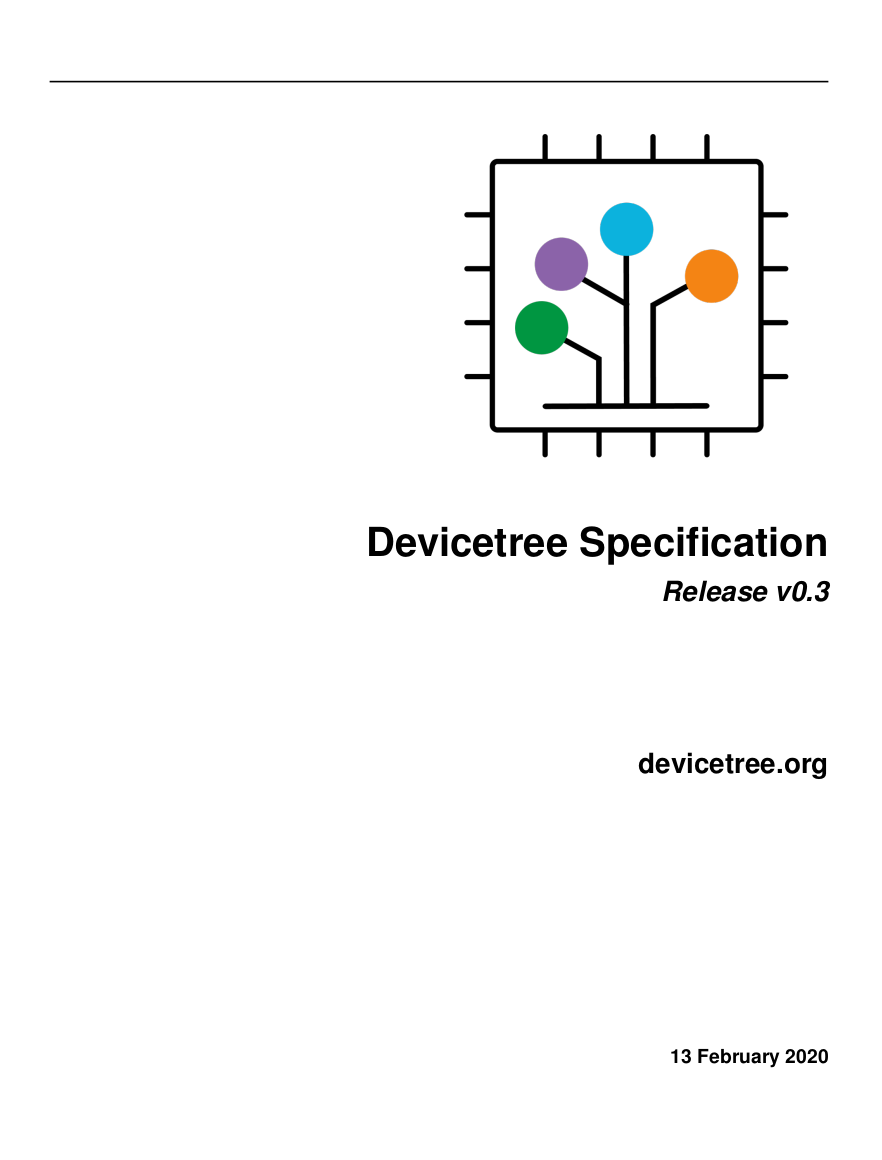
\includegraphics[width=\textwidth]{slides/linux-kernel-access-hw-dt/dt-spec.png}
  \end{columns}
\end{frame}

\begin{frame}[fragile]{Device Tree binding: old style}
  \begin{center}
    \kfile{Documentation/devicetree/bindings/mtd/spear_smi.txt}\\
    This IP is {\em not} used on STM32MP1.
  \end{center}
  \begin{columns}[t]
    \column{0.5\textwidth}
    \begin{block}{}
      {\fontsize{5}{6}\selectfont
\begin{verbatim}
* SPEAr SMI

Required properties:
- compatible : "st,spear600-smi"
- reg : Address range of the mtd chip
- #address-cells, #size-cells : Must be present if the device has sub-nodes
  representing partitions.
- interrupts: Should contain the STMMAC interrupts
- clock-rate : Functional clock rate of SMI in Hz

Optional properties:
- st,smi-fast-mode : Flash supports read in fast mode

\end{verbatim}
      }
    \end{block}
    \column{0.5\textwidth}
    \begin{block}{}
      {\fontsize{4}{5}\selectfont
\begin{verbatim}
Example:

        smi: flash@fc000000 {
                compatible = "st,spear600-smi";
                #address-cells = <1>;
                #size-cells = <1>;
                reg = <0xfc000000 0x1000>;
                interrupt-parent = <&vic1>;
                interrupts = <12>;
                clock-rate = <50000000>;        /* 50MHz */

                flash@f8000000 {
                        st,smi-fast-mode;
                        ...
                };
        };
\end{verbatim}
      }
    \end{block}
  \end{columns}

\end{frame}

\begin{frame}[fragile]{Device Tree binding: YAML style}
  \kfile{Documentation/devicetree/bindings/i2c/st,stm32-i2c.yaml}
  \begin{columns}[t]
    \column{0.5\textwidth}
    \begin{block}{}
      {\fontsize{5}{6}\selectfont
\begin{minted}{yaml}
# SPDX-License-Identifier: (GPL-2.0-only OR BSD-2-Clause)
%YAML 1.2
---
$id: http://devicetree.org/schemas/i2c/st,stm32-i2c.yaml#
$schema: http://devicetree.org/meta-schemas/core.yaml#

title: I2C controller embedded in STMicroelectronics STM32 I2C platform

maintainers:
  - Pierre-Yves MORDRET <pierre-yves.mordret@st.com>

properties:
  compatible:
    enum:
      - st,stm32f4-i2c
      - st,stm32f7-i2c
      - st,stm32mp15-i2c

  reg:
    maxItems: 1

  interrupts:
    items:
      - description: interrupt ID for I2C event
      - description: interrupt ID for I2C error

  resets:
    maxItems: 1

\end{minted}
      }
    \end{block}
    \column{0.5\textwidth}
    \begin{block}{}
      {\fontsize{5}{6}\selectfont
\begin{minted}{yaml}
  clocks:
    maxItems: 1

  dmas:
    items:
      - description: RX DMA Channel phandle
      - description: TX DMA Channel phandle

  ...

  clock-frequency:
    description: Desired I2C bus clock frequency in Hz. If not specified,
                 the default 100 kHz frequency will be used.
                 For STM32F7, STM32H7 and STM32MP1 SoCs, if timing
                 parameters match, the bus clock frequency can be from
                 1Hz to 1MHz.
    default: 100000
    minimum: 1
    maximum: 1000000

required:
  - compatible
  - reg
  - interrupts
  - resets
  - clocks
\end{minted}
      }
    \end{block}
  \end{columns}
\end{frame}

\begin{frame}[fragile]{Device Tree binding: YAML style example}
    \begin{block}{}
      {\fontsize{5}{6}\selectfont
\begin{minted}{yaml}
examples:
  - |
    //Example 3 (with st,stm32mp15-i2c compatible on stm32mp)
    #include <dt-bindings/interrupt-controller/arm-gic.h>
    #include <dt-bindings/clock/stm32mp1-clks.h>
    #include <dt-bindings/reset/stm32mp1-resets.h>
      i2c@40013000 {
          compatible = "st,stm32mp15-i2c";
          #address-cells = <1>;
          #size-cells = <0>;
          reg = <0x40013000 0x400>;
          interrupts = <GIC_SPI 33 IRQ_TYPE_LEVEL_HIGH>,
                       <GIC_SPI 34 IRQ_TYPE_LEVEL_HIGH>;
          clocks = <&rcc I2C2_K>;
          resets = <&rcc I2C2_R>;
          i2c-scl-rising-time-ns = <185>;
          i2c-scl-falling-time-ns = <20>;
          st,syscfg-fmp = <&syscfg 0x4 0x2>;
      };
\end{minted}
      }
    \end{block}
\end{frame}

\begin{frame}{Validating Device Tree in Linux}
  \begin{itemize}
  \item \code{dtc} only does syntactic validation
  \item YAML bindings allow to do semantic validation
  \item Linux kernel \code{make} rules:
    \begin{itemize}
    \item \code{make dt_binding_check}\\
      verify that YAML bindings are valid
    \item \code{make dtbs_check}\\
      validate DTs currently enabled against YAML bindings
    \item \code{make DT_SCHEMA_FILES=Documentation/devicetree/bindings/trivial-devices.yaml dtbs_check}\\
      validate DTs against a specific YAML binding
    \end{itemize}
  \end{itemize}
\end{frame}

\begin{frame}{The {\tt compatible} property}
  \begin{itemize}
  \item Is a list of strings
    \begin{itemize}
    \item From the most specific to the least specific
    \end{itemize}
  \item Describes the specific {\bf binding} to which the node complies.
  \item It uniquely identifies the {\bf programming model} of the
    device.
  \item Practically speaking, it is used by the operating system to
    find the {\bf appropriate driver} for this device.
  \item When describing real hardware, the typical form is
    \code{vendor,model}
  \item Examples:
    \begin{itemize}
    \item \code{compatible = "arm,armv7-timer";}
    \item \code{compatible = "st,stm32mp1-dwmac", "snps,dwmac-4.20a";}
    \item \code{compatible = "regulator-fixed";}
    \item \code{compatible = "gpio-keys";}
    \end{itemize}
  \item Special value: \code{simple-bus} $\rightarrow$ bus where all
    sub-nodes are memory-mapped devices
  \end{itemize}
\end{frame}

\begin{frame}{{\tt compatible} property and Linux kernel drivers}
  \begin{columns}
    \column{0.6\textwidth}
    \begin{itemize}
    \item Linux identifies as {\bf platform devices}:
      \begin{itemize}
      \item Top-level DT nodes with a \code{compatible} string
      \item Sub-nodes of \code{simple-bus}
        \begin{itemize}
        \item Instantiated automatically at boot time
        \end{itemize}
      \end{itemize}
    \item Sub-nodes of I2C controllers $\rightarrow$ {\em I2C devices}
    \item Sub-nodes of SPI controllers $\rightarrow$ {\em SPI devices}
    \item Each Linux driver has a table of compatible strings it supports
      \begin{itemize}
      \item \kstruct{of_device_id}\code{[]}
      \end{itemize}
    \item When a DT node compatible string matches a given driver, the
      device is {\em bound} to that driver.
    \end{itemize}
    \column{0.4\textwidth}
    \includegraphics[width=\textwidth]{slides/linux-kernel-access-hw-dt/dt-to-devices.pdf}
  \end{columns}
\end{frame}

\begin{frame}[fragile]{Matching with drivers in Linux: platform driver}
  \begin{block}{\kfile{drivers/tty/serial/stm32-usart.c}}
    {\tiny
\begin{minted}{c}
static const struct of_device_id stm32_match[] = {
        { .compatible = "st,stm32-uart", .data = &stm32f4_info},
        { .compatible = "st,stm32f7-uart", .data = &stm32f7_info},
        { .compatible = "st,stm32h7-uart", .data = &stm32h7_info},
        {},
};
MODULE_DEVICE_TABLE(of, stm32_match);

...

static struct platform_driver stm32_serial_driver = {
        .probe          = stm32_serial_probe,
        .remove         = stm32_serial_remove,
        .driver = {
                .name   = DRIVER_NAME,
                .pm     = &stm32_serial_pm_ops,
                .of_match_table = of_match_ptr(stm32_match),
        },
};
\end{minted}
    }
  \end{block}
\end{frame}

\begin{frame}[fragile]{Matching with drivers in Linux: I2C driver}
  \begin{block}{\kfile{sound/soc/codecs/cs42l51.c}}
    {\tiny
\begin{minted}{c}
const struct of_device_id cs42l51_of_match[] = {
        { .compatible = "cirrus,cs42l51", },
        { }
};
MODULE_DEVICE_TABLE(of, cs42l51_of_match);
\end{minted}
    }
  \end{block}
  \begin{block}{\kfile{sound/soc/codecs/cs42l51-i2c.c}}
    {\tiny
\begin{minted}{c}
static struct i2c_driver cs42l51_i2c_driver = {
        .driver = {
                .name = "cs42l51",
                .of_match_table = cs42l51_of_match,
                .pm = &cs42l51_pm_ops,
        },
        .probe = cs42l51_i2c_probe,
        .remove = cs42l51_i2c_remove,
        .id_table = cs42l51_i2c_id,
};
\end{minted}
    }
  \end{block}
\end{frame}

\begin{frame}[fragile]{{\tt reg} property}
  \begin{itemize}
  \item Most important property after \code{compatible}
  \item {\bf Memory-mapped} devices: base physical address and size of
    the memory-mapped registers. Can have several entries for multiple
    register areas.
\begin{onlyenv}<1>
\begin{block}{}
\begin{verbatim}
sai4: sai@50027000 {
    reg = <0x50027000 0x4>, <0x500273f0 0x10>;
};
\end{verbatim}
\end{block}
\end{onlyenv}
\pause
  \item {\bf I2C} devices: address of the device on the I2C bus.
\begin{onlyenv}<2>
\begin{block}{}
\begin{verbatim}
&i2c1 {
   hdmi-transmitter@39 {
      reg = <0x39>;
   };
   cs42l51: cs42l51@4a {
      reg = <0x4a>;
   };
};
\end{verbatim}
\end{block}
\end{onlyenv}
\pause
  \item {\bf SPI} devices: chip select number
\begin{onlyenv}<3>
\begin{block}{}
\begin{verbatim}
&qspi {
        flash0: mx66l51235l@0 {
                reg = <0>;
        };
        flash1: mx66l51235l@1 {
                reg = <1>;
        };
};
\end{verbatim}
\end{block}
\end{onlyenv}
\pause
\item The unit address must be the address of the first \code{reg}
  entry.
\begin{onlyenv}<4>
\begin{block}{}
\begin{verbatim}
sai4: sai@50027000 {
    reg = <0x50027000 0x4>, <0x500273f0 0x10>;
};
\end{verbatim}
\end{block}
\end{onlyenv}
  \end{itemize}
\end{frame}

\begin{frame}{Status property}
  \begin{itemize}
  \item The \code{status} property indicates if the device is really in
    use or not
    \begin{itemize}
    \item \code{okay} or \code{ok} $\rightarrow$ the device is really
      in use
    \item any other value, by convention \code{disabled} $\rightarrow$
      the device is not in use
    \end{itemize}
  \item In Linux, controls if a device is instantiated
  \item In \code{.dtsi} files describing SoCs: all devices that
    interface to the outside world have \code{status = "disabled";}
  \item Enabled on a per-device basis in the board \code{.dts}
  \end{itemize}
\end{frame}

\begin{frame}[fragile]{Resources: interrupts, clocks, DMA, reset lines, ...}
  \begin{columns}
  \column{0.5\textwidth}
  \begin{itemize}
  \item Common pattern for resources shared by multiple hardware
    blocks
    \begin{itemize}
    \item Interrupt lines
    \item Clock controllers
    \item DMA controllers
    \item Reset controllers
    \item ...
    \end{itemize}
  \item A Device Tree node describing the {\em controller} as a device
  \item References from other nodes that use resources provided by
    this {\em controller}
  \end{itemize}
  \column{0.5\textwidth}
\begin{block}{}
{\tiny
\begin{minted}{perl}
intc: interrupt-controller@a0021000 {
   compatible = "arm,cortex-a7-gic";
   #interrupt-cells = <3>;
   interrupt-controller;
   reg = <0xa0021000 0x1000>, <0xa0022000 0x2000>;
};

rcc: rcc@50000000 {
   compatible = "st,stm32mp1-rcc", "syscon";
   reg = <0x50000000 0x1000>;
   #clock-cells = <1>;
   #reset-cells = <1>;
};

dmamux1: dma-router@48002000 {
   compatible = "st,stm32h7-dmamux";
   reg = <0x48002000 0x1c>;
   #dma-cells = <3>;
   clocks = <&rcc DMAMUX>;
   resets = <&rcc DMAMUX_R>;
};

spi3: spi@4000c000 {
   interrupts = <GIC_SPI 51 IRQ_TYPE_LEVEL_HIGH>;
   clocks = <&rcc SPI3_K>;
   resets = <&rcc SPI3_R>;
   dmas = <&dmamux1 61 0x400 0x05>,  <&dmamux1 62 0x400 0x05>;
};
\end{minted}
}
\end{block}
\end{columns}
\end{frame}

\begin{frame}{Pin-muxing description}
  \begin{columns}
    \column{0.5\textwidth}
    \begin{itemize}
    \item Most modern SoCs, including the STM32MP1, have more features
      than they have pins to expose those features to the outside world.
    \item Pins are muxed: a given pin can be used for one function
      {\bf or} another
    \item A specific IP block in the SoC controls the muxing of pins:
      the {\bf pinmux controller}
    \item The Device Tree describes which pin configurations are
      possible, and which configurations are used by the different
      devices.
    \end{itemize}
    \column{0.5\textwidth}
    \includegraphics[width=\textwidth]{slides/linux-kernel-access-hw-dt/pin-muxing-principle.pdf}
  \end{columns}
\end{frame}

\begin{frame}[fragile]{Pin-muxing controllers on STM32MP1}
  \begin{block}{\kfileversion{arch/arm/boot/dts/stm32mp151.dtsi}{6.1}}
{\tiny
\begin{minted}{perl}
pinctrl: pin-controller@50002000 {
        #address-cells = <1>;
        #size-cells = <1>;
        compatible = "st,stm32mp157-pinctrl";
        ...
        gpioa: gpio@50002000 { ... };
        gpiob: gpio@50003000 { ... };
        gpioc: gpio@50004000 { ... };
        gpiod: gpio@50005000 { ... };
        gpioe: gpio@50006000 { ... };
        gpiof: gpio@50007000 { ... };
        ...
};

pinctrl_z: pin-controller-z@54004000 {
        #address-cells = <1>;
        #size-cells = <1>;
        compatible = "st,stm32mp157-z-pinctrl";
        ranges = <0 0x54004000 0x400>;
        ...
        gpioz: gpio@54004000 { .... };
        ...
};
\end{minted}
}
  \end{block}
\end{frame}

\begin{frame}[fragile]{Pin-muxing configuration}
\begin{onlyenv}<1>
  \begin{block}{\kfile{arch/arm/boot/dts/stm32mp15-pinctrl.dtsi}}
{\tiny
\begin{minted}{perl}
&pinctrl {
        ...
        i2c1_pins_a: i2c1-0 {
                pins {
                        pinmux = <STM32_PINMUX('D', 12, AF5)>, /* I2C1_SCL */
                                 <STM32_PINMUX('F', 15, AF5)>; /* I2C1_SDA */
                        bias-disable;
                        drive-open-drain;
                        slew-rate = <0>;
                };
        };
        ...
        m_can1_pins_a: m-can1-0 {
                pins1 {
                        pinmux = <STM32_PINMUX('H', 13, AF9)>; /* CAN1_TX */
                        slew-rate = <1>;
                        drive-push-pull;
                        bias-disable;
                };
                pins2 {
                        pinmux = <STM32_PINMUX('I', 9, AF9)>; /* CAN1_RX */
                        bias-disable;
                };
        };
        ...
};
\end{minted}
}
  \end{block}
\end{onlyenv}
\begin{onlyenv}<2>
  \begin{center}
    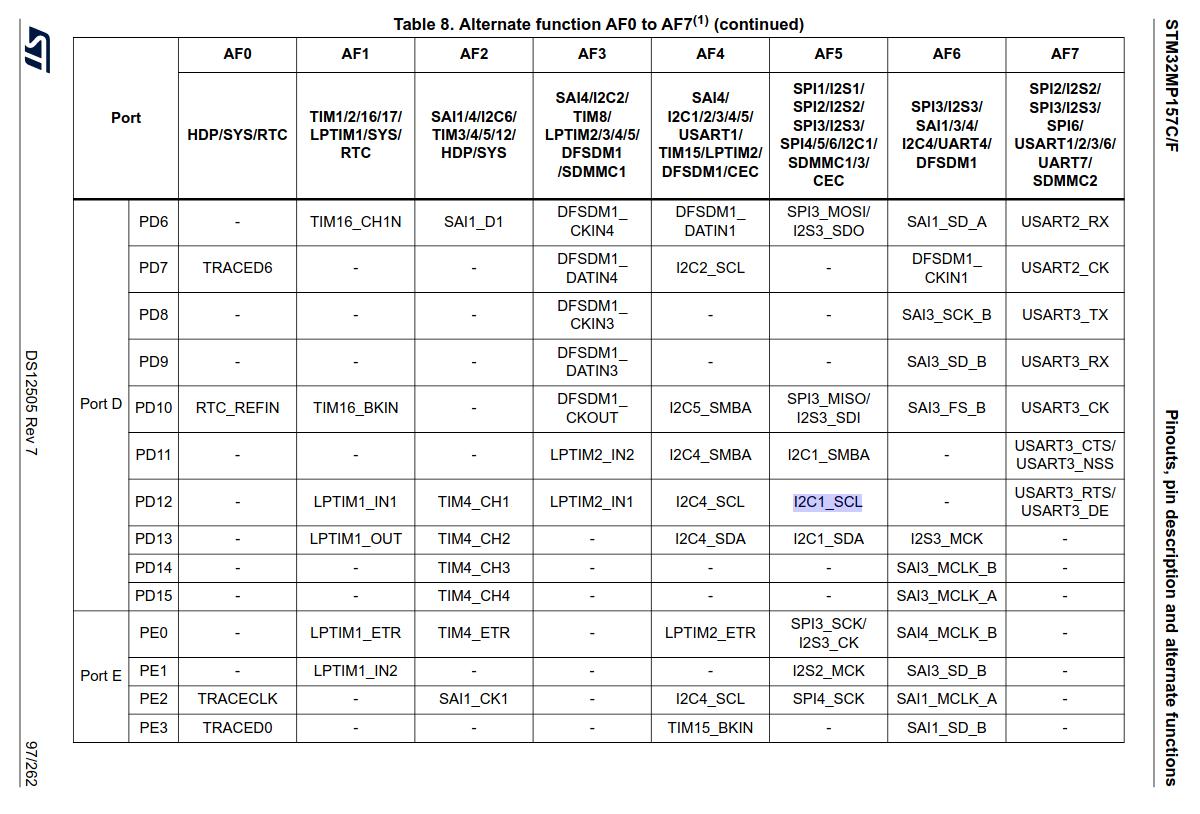
\includegraphics[height=0.78\textheight]{slides/linux-kernel-access-hw-dt/stm32mp157-i2c-pin-mux.png}
  \end{center}
  \tiny
  Source: \href{https://www.st.com/resource/en/datasheet/stm32mp157c.pdf}{STM32MP157C
  datasheet}. Note that \code{I2C1_SDA} is also available on pin \code{PF15} (not shown here).
\end{onlyenv}
\end{frame}

\begin{frame}[fragile]{Pin-muxing consumer}
  \begin{block}{}
{\tiny
\begin{minted}{perl}
&i2c1 {
        pinctrl-names = "default", "sleep";
        pinctrl-0 = <&i2c1_pins_a>;
        pinctrl-1 = <&i2c1_sleep_pins_a>;
        ...
};
\end{minted}
}
\end{block}
\begin{itemize}
\item Typically board-specific, in \code{.dts}
\item \code{pinctrl-0}, \code{pinctrl-1}, \code{pinctrl-X} provides
  the pin mux configurations for the different {\bf states}
\item \code{pinctrl-names} gives a name to each state, mandatory even
  if only one state
\item States are mutually exclusive
\item The driver is responsible for switching between states
\item \code{default} state is automatically set up when the device is
  {\em probed}
\end{itemize}
\end{frame}

\begin{frame}[fragile]{Example: LED and I2C device}
  \begin{itemize}
  \item Let's see how to describe an LED and an I2C device connected
    to the DK1 platform.
  \item Create \code{arch/arm/boot/dts/stm32mp157a-dk1-custom.dts}
    which includes \code{stm32mp157a-dk1.dts}
    \begin{block}{}
{\tiny
\begin{verbatim}
#include "stm32mp157a-dk1.dts"
\end{verbatim}
}
    \end{block}
  \item Make sure \code{stm32mp157a-dk1-custom.dts} gets compiled to a
    DTB by changing \kfile{arch/arm/boot/dts/Makefile}
    \begin{block}{}
      {\tiny
\begin{verbatim}
dtb-$(CONFIG_ARCH_STM32) += \
        ...
        stm32mp157a-dk1.dtb \
        stm32mp157a-dk1-custom.dtb \
\end{verbatim}
      }
    \end{block}
  \item \code{make dtbs}
    \begin{block}{}
      {\tiny
\begin{verbatim}
  DTC     arch/arm/boot/dts/stm32mp157a-dk1-custom.dtb
\end{verbatim}
      }
    \end{block}
  \end{itemize}
\end{frame}

\begin{frame}[fragile]{Example: describe an LED}
  \begin{columns}
    \column{0.5\textwidth}
  \begin{block}{stm32mp157a-dk1-custom.dts}
    {\tiny
\begin{minted}{perl}
#include "stm32mp157a-dk1.dts"

/ {
        leds {
                compatible = "gpio-leds";
                webinar {
                        label = "webinar";
                        gpios = <&gpioe 1 GPIO_ACTIVE_HIGH>;
                };
        };
};
\end{minted}
      }
  \end{block}
  \begin{block}{shell}
{\tiny
\begin{verbatim}
# echo 255 > /sys/class/leds/webinar/brightness
\end{verbatim}
}
\end{block}
  \column{0.5\textwidth}
  \begin{center}
    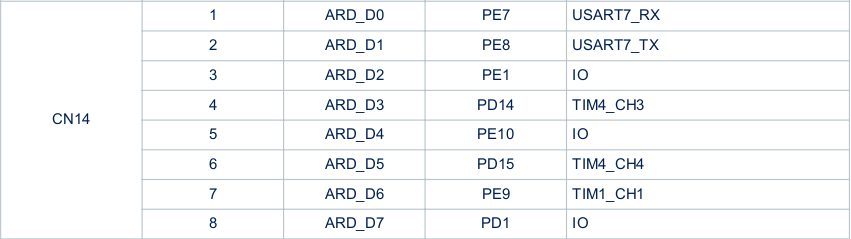
\includegraphics[width=1\textwidth]{slides/linux-kernel-access-hw-dt/cn14-pinout.png}\\
    \vspace{0.5cm}
    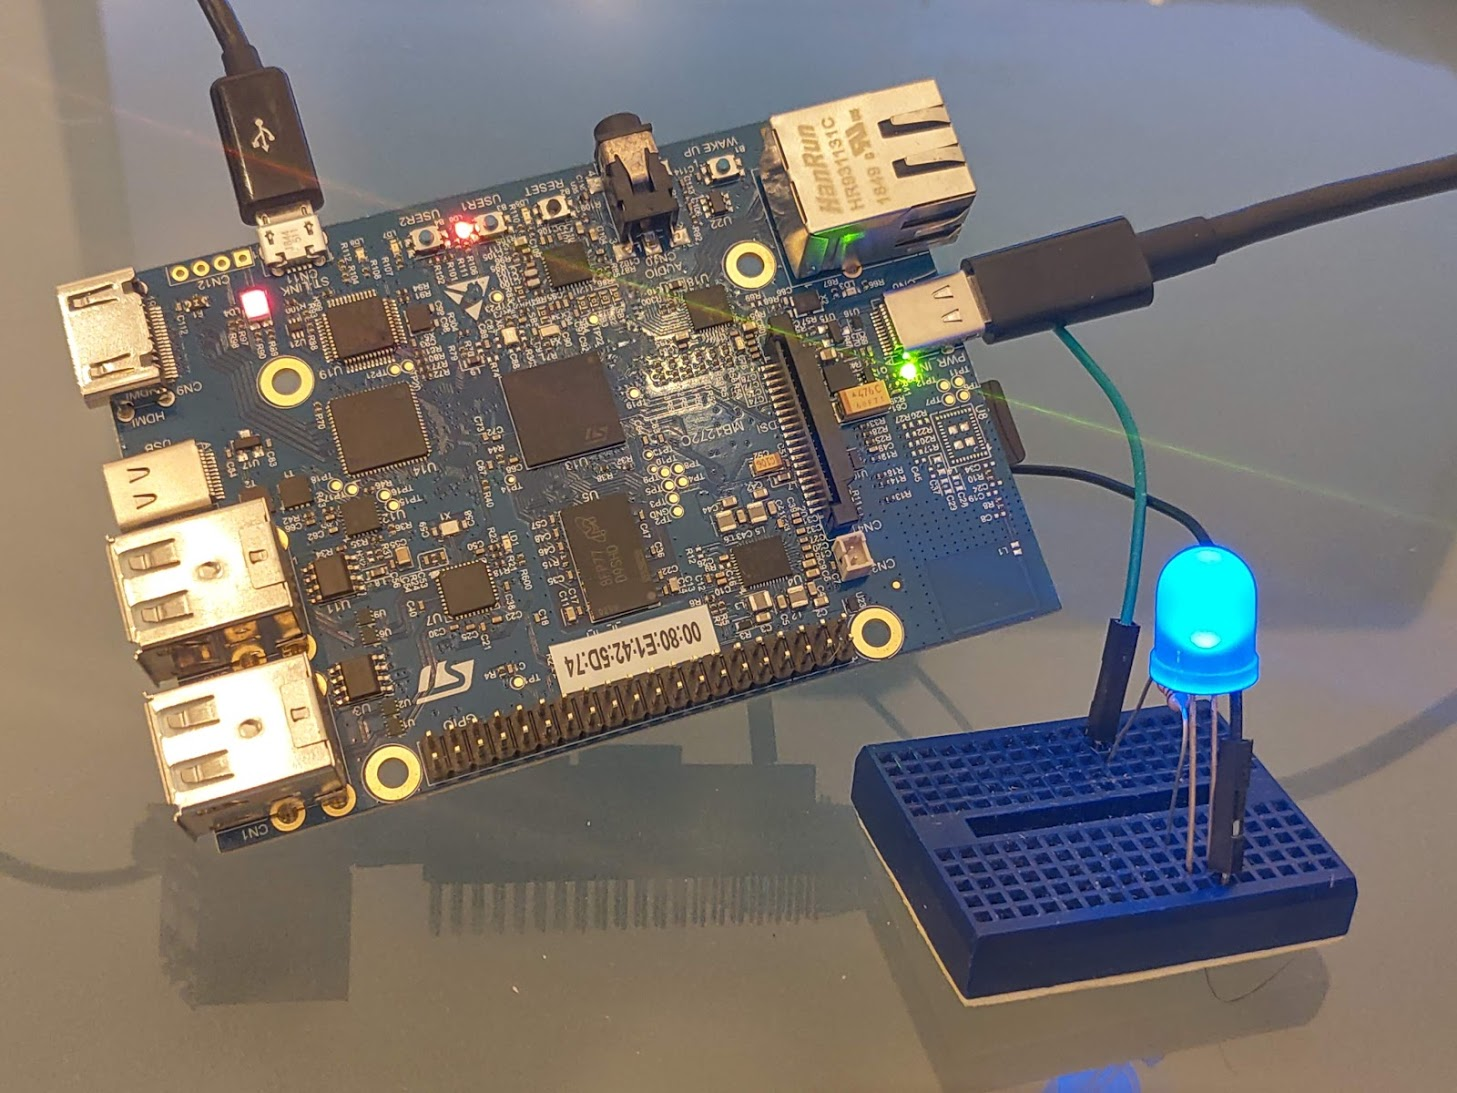
\includegraphics[height=0.3\textheight]{slides/linux-kernel-access-hw-dt/led-on.jpg}
  \end{center}
  \end{columns}
\end{frame}

\begin{frame}[fragile]{Example: connect I2C temperature, humidity and pressure sensor}
  \begin{columns}
    \column{0.5\textwidth}
    \begin{block}{stm32mp157a-dk1-custom.dts}
      {\tiny
\begin{minted}{perl}
&i2c5 {
        status = "okay";
        clock-frequency = <100000>;
        pinctrl-names = "default", "sleep";
        pinctrl-0 = <&i2c5_pins_a>;
        pinctrl-1 = <&i2c5_pins_sleep_a>;

        pressure@76 {
                compatible = "bosch,bme280";
                reg = <0x76>;
        };
};
\end{minted}
}
  \end{block}

\begin{block}{shell}
{\tiny
\begin{verbatim}
# cat /sys/bus/iio/devices/iio\:device2/in_humidityrelative_input
49147
# cat /sys/bus/iio/devices/iio\:device2/in_pressure_input
101.567167968
# cat /sys/bus/iio/devices/iio\:device2/in_temp_input
24380
\end{verbatim}
}
\end{block}
  \column{0.5\textwidth}
  \begin{center}
    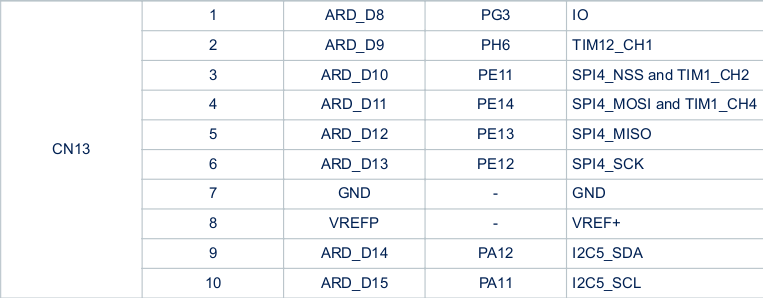
\includegraphics[width=\textwidth]{slides/linux-kernel-access-hw-dt/cn13-pinout.png}\\
    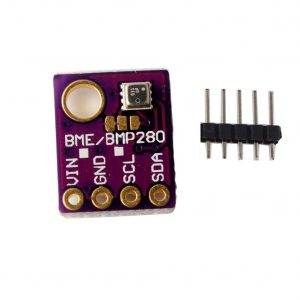
\includegraphics[width=0.4\textwidth]{slides/linux-kernel-access-hw-dt/bme.jpg}
  \end{center}
\end{columns}
\vspace{0.5cm}
Details at
\url{https://bootlin.com/blog/building-a-linux-system-for-the-stm32mp1-connecting-an-i2c-sensor/}
\end{frame}

\begin{frame}{Further details about the Device Tree}
\small
Check out our {\em Device Tree 101 webinar}, by Thomas Petazzoni (2021)
\begin{itemize}
    \item Slides: \url{https://bootlin.com/blog/device-tree-101-webinar-slides-and-videos/}\\
    \item Video: \url{https://youtu.be/a9CZ1Uk3OYQ}
\end{itemize}
\vspace{0.5cm}
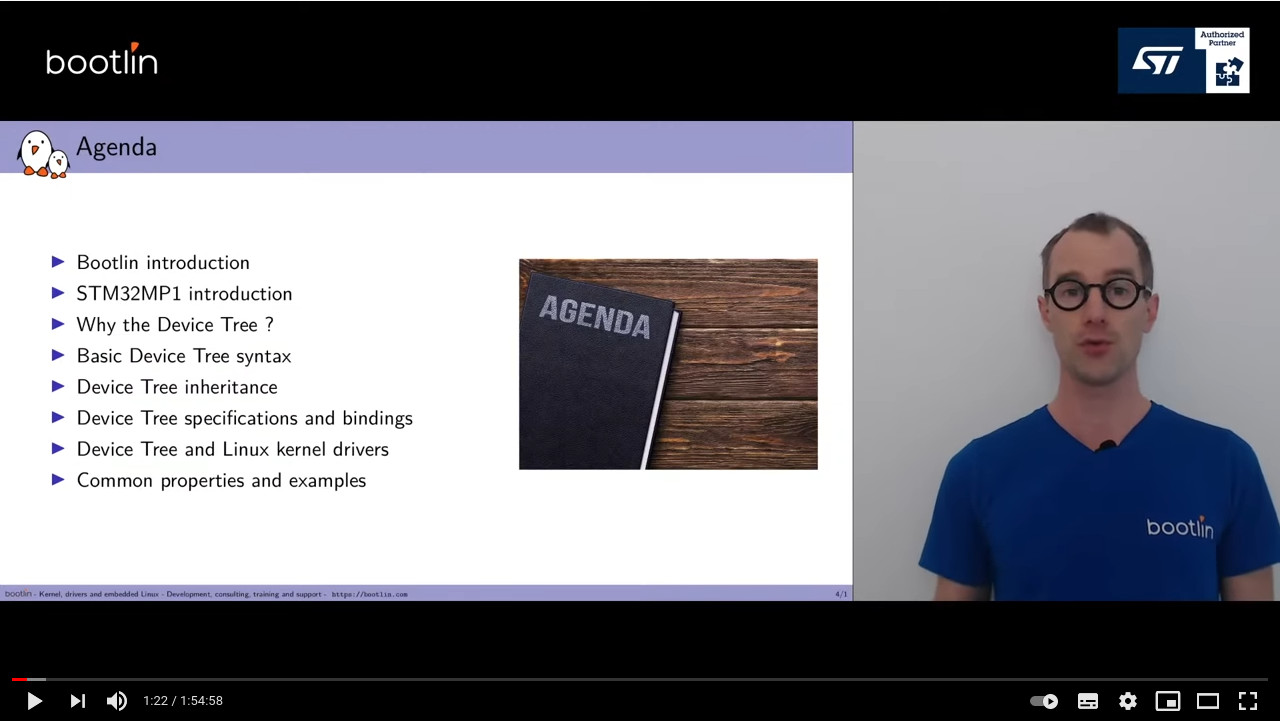
\includegraphics[height=0.5\textheight]{common/pictures/device-tree-video.jpg}
\end{frame}
